\documentclass{standalone}
\usepackage{tikz}
\begin{document}
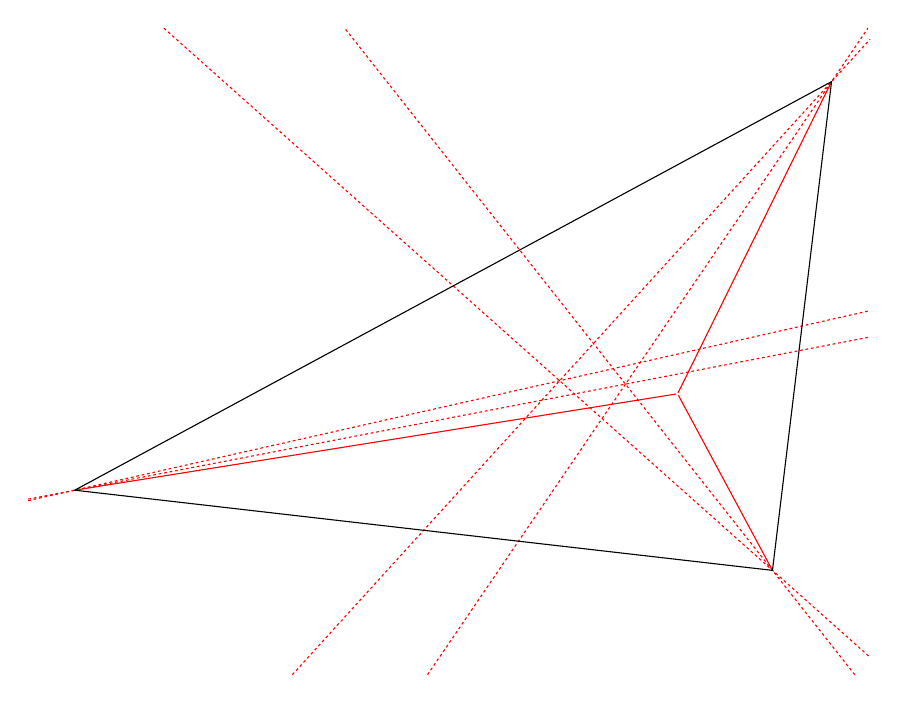
\begin{tikzpicture}[x=1pt,y=1pt]
\draw[red, dash pattern=on 1pt] (296.76,-231.73) -- (112.45,1.87);
\draw[red, dash pattern=on 1pt] (142.38,-231.73) -- (301.51,1.87);
\draw[red, dash pattern=on 1pt] (-1.91,-168.30) -- (302.29,-109.70);
\draw[red, dash pattern=on 1pt] (93.52,-231.73) -- (302.29,-2.11);
\draw[red, dash pattern=on 1pt] (47.13,1.87) -- (302.29,-225.44);
\draw[red, dash pattern=on 1pt] (-1.91,-168.85) -- (302.29,-100.18);
\draw[red] (16.04,-164.88) -- (232.16,-130.31);
\draw[red] (266.76,-193.55) -- (233.02,-130.75);
\draw[red] (232.90,-129.90) -- (288.05,-18.06);
\draw (14.90,-165.06) -- (267.02,-194.03) -- (288.37,-17.43) -- cycle;
\end{tikzpicture}
\end{document}
